\section{Nuclear Scattering Reactions in the Glauber Framework}
Explain path to go:
\begin{itemize}
\item short intro why we use scrattering reactions: to study structure of nuclei (mostly via e. scattering as they only interact via electromagn. force) and refer to chapter. Introduce problems qe account body problem etc
\item starting from elastic scattering at low energies going to medium to high energies
\itemexplain glauber: eikonal wave approximations, optical limit which leads to optical potential model, description via nucleon nucleon interaction
\end{itemize}
\subsection{Elastic scattering at low energies}
\begin{itemize}
\item Rutherford scattering→ poiniering works (alpha particle on gold atoms) – description in classical mechanics
\item Rutherford scattering only valid if coulomb potential
\item at low energies below pion production only elastic cross section
\item introduce here the Scattering problem in quantum mechanics (see Schindler, p. 23)
\item from classical physics we go to quantum mechanics and use partial wave decomposition with theta being the scattering angle
\item include in this picture coulomb and nuclear interaction (as done in Kuk, page 120)
\end{itemize}
\subsection{Nuclear Density distribution studies via elastic scattering}
\begin{itemize}
\item Rutherford, Mott and Rosenbluth
\item  show something about form Factors
\item  are charge radii and nuclear radii measured?
\item note approximation for $^{12}C$ that neutron radius same as proton radius
\end{itemize}
\subsection{Glauber Model for nuclear scatering at high energies}
\begin{itemize}
\item explain model assumption
\item eikonal wave approximation: high incoming momentum,low scattering angle
\item Show picture of scattering
\item optical limit: - Nucleons at high energy → undeflected due to large momentum (linear trajectory)
		   -Nucleus large compared to nucleon-nucleon  force
		   -Motion of nucleons independent of nucleus
		   -overall cross-section described in terms of nucleon-nucleon cross section
\item Description in the Probability Approach (also here I use all the eiconal and optical limit approximation)
\item Description in the Eikonal optical-limit approximation
\item Comparison of both descriptions methods  for tota interaction cross section→ should end up with same. Advantage of PA is that you can calculate the cross section for a defined number of removed projectile nucleons (Schindler, p. 49)
\end{itemize}
\subsubsection{Extensions to the Glauber model}
\begin{itemize}
\item things which cannot be neglected and influence the cross section
\item in medium modifications (see Lukas thesis)
\item Coulomb interaction
\item Pauli blocking
\end{itemize}
\subsection{Cross sections for $^{12}C + ^{12}C$}
\begin{itemize}
\item Total reaction cross section
\item charge changing cross section → maybe I have to include lise++ calculations
\item isotope corrections- neutron removal → maybe I have to include lise++ calculations
\end{itemize}

\subsection{Quasi-Free Scattering (QFS) Reactions}
Quasi-free scattering (QFS) reactions, as a subset of direct reactions, are processes where a projectile nucleon interacts with a target nucleon in a single, fast, and highly localized event. The timescale of these interactions is extremely short, approximately $10^{-21}$ s, implying that the relative kinetic energies of the participants are high, typically $\gtrsim$ 100 AMeV.\newline
In QFS experiments conducted in direct kinematics, a proton serves as the projectile, colliding with a nucleon or a cluster within the target nucleus. Conversely, in inverse kinematics, the nucleus of interest becomes the projectile, while a proton or proton-like particle is used as the target. Despite these differing setups, both approaches are fundamentally equivalent, differing only due to a Lorentz transformation of the reference frame.\newline
As the name implies, QFS reactions are conceptually similar to free nucleon-nucleon scattering, with the primary approximation being that the influence of the residual nucleus is neglected to first order. This approximation simplifies the theoretical description of the process, allowing to treat the interaction as a two-body problem within a (only weakly interfering) nuclear environment.\newline
The first experiments confirming the existence of quasi-free scattering processes were conducted at the University of California, Berkeley, in 1952 by O. Chamberlain and Emilio Segr\`e\cite{chamberlain1952proton}. In their study, lithium nuclei were bombarded with 350 MeV protons, and coincident proton pairs were observed with an opening angle of approximately 90$^{\circ}$. That same year, J.B. Cladis, W.N. Hess, and B.J. Moyer published results on the scattering of 340 MeV protons on deuterium and carbon targets\cite{cladis1952nucleon}, further substantiating the phenomenon.\newline
In 1957, Tyren, Maris, and Hillman designed an experiment aimed at fully characterizing proton-proton collisions within the quasi-free scattering framework\cite{MARIS19581}. Their results validated the assumption of a direct and clean interaction between the projectile and the target nucleon, free from significant distortions caused by the surrounding nucleus. Furthermore, these experiments demonstrated that QFS reactions could serve as a powerful tool for probing nuclear structure and testing predictions of the shell model. Specifically, they enabled the study of key nuclear parameters such as spin-orbit splitting and energy differences between nuclear shells and here fore to probe the shell evolution. \newline
In QFS reactions, these parameters can be extracted by analyzing the reaction products, which include the two correlated outgoing protons, the residual nucleus, and any gamma rays emitted during de-excitation of the residual nucleus. The detailed measurements of these observables provide critical insights into the underlying nuclear structure and dynamics.\newline
The experimental discoveries and theoretical insights from these early studies catalyzed significant advancements in the theoretical modeling of QFS reactions. These models have since become essential tools for understanding nucleon-nucleon interactions within the nuclear medium and for refining our knowledge of nuclear structure and reaction mechanisms.\newline
\subsubsection{Kinematics of QFS Reactions}\label{sec:kin_qfs}
A simplified picture, which however explains the essential physics of the QFS reaction, can be found in figure \ref{fig:sketch_qfs}: we have an incoming proton knocking out a nuclear constituent (proton/neutron) in a free nucleon-nucleon collision ending with a final state having the scattered proton, the scattered  off nuclear constituent and the rest nucleus (A-1)$^*$. In this picture index \textit{0} is assigned to the incoming proton, \textit{1} to the knocked out nucleon, \textit{2} to the outgoing projectile proton, \textit{A} to the initial nucleus and  \textit{A-1} to the final nucleus accordingly.
\begin{figure}[htpb]
    \centering
    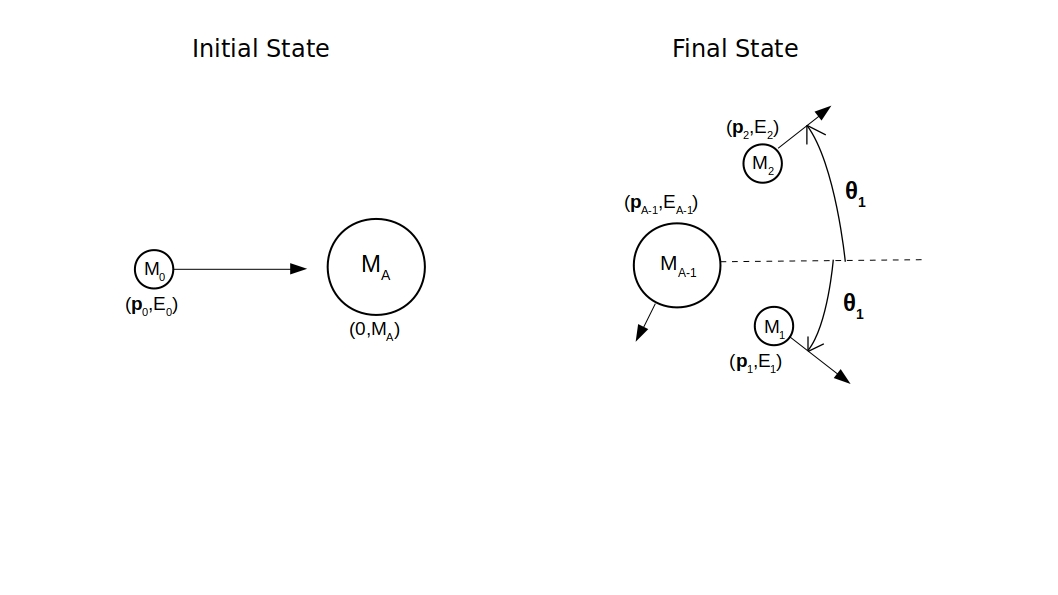
\includegraphics[width=\textwidth,height=8cm,keepaspectratio=true]{Figures/sketch_qfs.jpg}
    \caption{
   	Simplified picture of the QFS reaction process in direkt kinematics.  
    }
    \label{fig:sketch_qfs}
\end{figure}
From energy -momentum conservation the reaction can be expressed as:
\begin{equation}\label{eq:four_mom_cons_qfs}
P_A  +  P_0 = P_1 + P_2 +P_{A-1} 
\end{equation}
with $P_i$ the four momentum $(\mathbf{p_i},E_i)$.\newline
In direct kinematics as presented in figure \ref{fig:sketch_qfs} the separation of the ejected nucleon for a certain final state of the nucleus \textit{A-1} is given by\footnote{In inverse kinematics the four-momentum vectors need to be boosted to the center of mass frame of the initial nucleus via Lorentz transformation.}:
\begin{equation}
S = T_0 -(T_1+T_2 +T_{A-1}); \; \text{with $T_i$ the kinetic energy of particle $i$} 
\label{eq:sep_e}
\end{equation}
In the idealized shell model the separation energy equals to the (negative) energy of the nucleus' single-particle state. For the case the proton knocks out the least bound nucleon (proton/neutron) the final nucleus is lying in the ground state with $E_{A-1} = M_{A-1}c^2  + T_{A-1}$.\newline
If a nucleon has been ejected from an inner shell resulting in a hole state, the final nucleus will be in an excited state:
\begin{equation}
E^{*}_{A-1} =  M_{A-1}c^2  +T_{A-1} + E_{exe}
\end{equation} 
The excitation energy $E_{exe}$ is reflected in the difference in the separation energy of the least bound nucleon and the ejected one. From the experimental point of view $E_{exe}$ is directly accessible via gamma detection from the transition of the final nucleus from the excited to the ground state. 
According to the picture of having a nucleon nucleon scattering process with no influence of the residual nucleus A-1 we can approximate $\mathbf{p_A} \approx \mathbf{p_i} + \mathbf{p_{A-1}}$ where $\mathbf{p_i}$ is the initial nucleon momentum inside the initial nucleus A. Since the initial nucleus is at rest ($\mathbf{p_A} = 0$), the recoil momentum of the nucleus in final state $\mathbf{p_{A-1}}$ equals to $-\mathbf{p_i}$ the momentum of the initial nucleon pointing in opposite direction. \newline
In addition the four-momentum of the inner nucleon can be deduced from momentum measurement of the initial and final state free nucleons:
\begin{equation}
P_i \approx P_{miss} \equiv P_1 + P_2  - P_0
\end{equation}
where $P_{miss}$ is the so called "measured missing four-momentum of the reaction"\cite{patsyuk2021unperturbed}\footnote{$P_{miss}$ is only equal to $P_i$ for the unperturbed QFS (no ISI/FSI) case.}.
Thereupon, the separation energy measurement and the recoil momentum distribution fully describe the single paricle state in the various shell levels. 
In addition and as complementary method $\gamma$ rays can be measured in coincidence with the reaction and consequentely exclusive cross section and momentum distribution measurements of the single particle states are accessible as illustrated in figure blabla.\newline
Considering the removal of a single nucleon from an initial nucleus with A nucleons and initial spin \textit{I} $\Psi^A_i$ and final nucleus state  $\Psi^{A-1}_f$ with final spin $I_f$ an overlap function between intial and final state many-body wave function can be written as:
\begin{equation}
\langle \vec{r}, \Psi_f^{A^{-1}} | \Psi_i^A \rangle = \sum_j C_j^{if} \psi_j(\vec{r}), \quad with  |I - I_f| < j < |I + I_f|
\end{equation}
where $S_j^{if} = |C_j^{if}|^2$ is the commonly named spectroscopic factor, see ref \cite{hansen2003direct} sec.2.1. $S_j^{if}$ is summed over all final single particle states m (from $-j$ to $j$). It is unity for nucleon removal from a pure single particle state and equals (2j+1) when the nucleon was removed from a filled j-subshell.
The spectroscopic factor is linked to the exclusive experimental cross section measurement of a single particle state and the theoretical predicted one, as in ref \cite{hansen2003direct}:
\begin{equation}
\sigma_{th}^{if} = \sum_j S_j^{if}\,\sigma_{sp}(nlj)
\end{equation}
where $\sigma_{sp}$ are the theoretical cross sections for the normalized wave functions $\Psi_j$ of the final state nucleus A-1 with the appropriate quantum numbers.\newline
From this considerations the spectroscopic factor can be used to probe the theoretical shell predictions. In past this was already done with direct qfs-reactions $(e,e'p)$. Results for the spectroscopic factor with data obtained at the NIKHEF facility is shown in figure \ref{fig:spec_fac}. The substantial reduction of the spectroscopic factor with respect to the independent particle model (IPM) or mean field of $\approx 35\%$ indicates a substantial depletion of the single-hole states and inferring from this a refined model prediction has to be applied\footnote{The mean field potential does not consider spin-spin interaction $V_{ss}$, non central tensor-potential $V_T$ or spin-orbit interaction $V_{LS}$.}.\newline
\begin{figure}[h!]
    \centering
    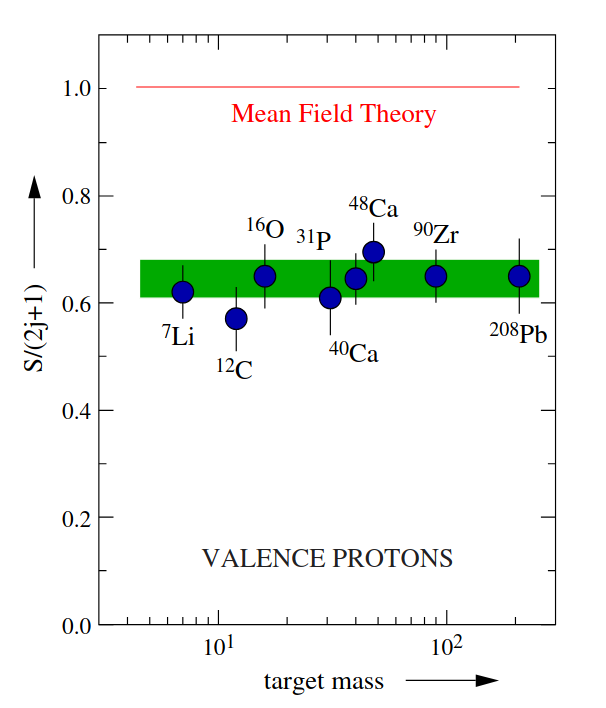
\includegraphics[width=\textwidth,height=8cm,keepaspectratio=true]{Figures/spec_factor.png}
    \caption{Normalized spectroscopic factors from the $(e, e\prime p)$ reaction as a function of target mass taken from \cite{DICKHOFF2004377}. As input for the theoretical cross sections the prediction from mean field models were used. }
    \label{fig:spec_fac}
\end{figure}
While qfs-reaction with electrons $(e,e\prime p)$ in direct kinematics is a valuable method to make precise measurements for stable (target) nuclei it is not suitable for the experimental analysis with exotic (neutron or proton rich) nuclei. Due to their unstability they have a short lifetime (e.g. $^{52}Ca$ with $\tau = 4.6s$) they can hardly serve as targets. Inducing the reaction in inverse kinematics - having electrons as targets and the exotic nuclei of interest as projectiles - is also not feasible since no free electons can be captured as target. The alternative approach is to use proton induced quasi-free scattering in inverse kinematics where the exotic beam inpinges on an extended proton target such as liquid hydrogen $H_2$  or a fixed proton rich target such as $CH_2$\footnote{Herefore a carbon target reference run is used to extract the qfs-reaction events from the $CH_2$ target run.}.\newline
Summarizing, the qfs-reaction technique in inverse kinematics with exotic nuclei as in-flight projectiles and a proton-like target opens new possibilities to probe theoretical model predictions of deformed nuclei far off stability which haven't been accessible before.\newline
For precise cross section measurements of the single particle states $\sigma_{sp}$ the kinematical characteristics of the qfs-reaction products have to be considered for correct identification of qfs-events and clear background substraction. The following descriptions are already encoded in equation \ref{eq:four_mom_cons_qfs}.\newline
As starting point one compares the qfs-reaction of the two nucleons with the two dimensionali non-central collision of free pointlike particles in nonrelativistic kinematics. Since both kinetic energy and momenta are conserved a  clear signature is expected: the opening angle of the scattered particles is exactly 90 \textdegree. 

From experimental point of view-> important to identify the QFS events.
In non rel. kinematics of free particles a really clean signature: two dim-colllision with coplanar nucleons = delta phi = 180 degr and an opening angle of 90 degr. \newline
When going to rel. energies -> 80 degrees of opening angle(400 AMeV). Is there a function to calculate the opening angle? The opening angle is smeared because of relativistic effects + inner momentum of the nucleon. \newline
Explain Goldhaber model to characterize the width of the inner momenta.\newline
Plot the correlation plots of opening angle and delta phi.
Then mentnion pronounced transversal correlation as in L.V. Chulkov -> insert image
Moreover limited energy ranges are allowed where the forward nucleon has much higher energy compared to the larger scattered one -> insert image


\subsubsection{Cross Sections for QFS Reactions - Qualitative Considerations}
see more in the standard work, TO BE DONE
\subsubsection{Application Fields of QFS Reactions}
As already mentioned in section \ref{sec:kin_qfs}, for to determine the spectroscopic strength = cross sec x spectroscopic factor, where you get the cross section from the Glauber reaction Model and the spectroscopic factor from the according shell model/interactions
We see a systematic quenching.
\newline
Gammma Spectroscopy:
especially the first excited 2+ state of special interest, gives info about structure and deformation of the nucleus. Write here a little bit more and make research if you can find something\newline
QFS reactions to probe clustering and nuclear halos:
\newline
Population of unbound nuclei and states: to read, still unclear..\newline

Study of NN interaction (SRC,LRC etc) \newline

Fission via quasi free scattering -> highlight this one. Here write more about it...
\newline



